
\documentclass[journal,12pt,twocolumn]{IEEEtran}

\usepackage{setspace}
\usepackage{gensymb}
\usepackage{float}
\singlespacing


\usepackage[cmex10]{amsmath}

\usepackage{amsthm}

\usepackage{mathrsfs}
\usepackage{txfonts}
\usepackage{stfloats}
\usepackage{bm}
\usepackage{cite}
\usepackage{cases}
\usepackage{subfig}

\usepackage{longtable}
\usepackage{multirow}

\usepackage{enumitem}
\usepackage{mathtools}
\usepackage{steinmetz}
\usepackage{tikz}
\usepackage{circuitikz}
\usepackage{verbatim}
\usepackage{tfrupee}
\usepackage[breaklinks=true]{hyperref}
\usepackage{graphicx}
\usepackage{graphics}
\usepackage{tkz-euclide}
\usepackage{float}

\usetikzlibrary{calc,math}
\usepackage{listings}
    \usepackage{color}                                            %%
    \usepackage{array}                                            %%
    \usepackage{longtable}                                        %%
    \usepackage{calc}                                             %%
    \usepackage{multirow}                                         %%
    \usepackage{hhline}                                           %%
    \usepackage{ifthen}                                           %%
    \usepackage{lscape}     
\usepackage{multicol}
\usepackage{chngcntr}

\DeclareMathOperator*{\Res}{Res}

\renewcommand\thesection{\arabic{section}}
\renewcommand\thesubsection{\thesection.\arabic{subsection}}
\renewcommand\thesubsubsection{\thesubsection.\arabic{subsubsection}}

\renewcommand\thesectiondis{\arabic{section}}
\renewcommand\thesubsectiondis{\thesectiondis.\arabic{subsection}}
\renewcommand\thesubsubsectiondis{\thesubsectiondis.\arabic{subsubsection}}


\hyphenation{op-tical net-works semi-conduc-tor}
\def\inputGnumericTable{}                                 %%

\lstset{
%language=C,
frame=single, 
breaklines=true,
columns=fullflexible
}
\begin{document}


\newtheorem{theorem}{Theorem}[section]
\newtheorem{problem}{Problem}
\newtheorem{proposition}{Proposition}[section]
\newtheorem{lemma}{Lemma}[section]
\newtheorem{corollary}[theorem]{Corollary}
\newtheorem{example}{Example}[section]
\newtheorem{definition}[problem]{Definition}

\newcommand{\BEQA}{\begin{eqnarray}}
\newcommand{\EEQA}{\end{eqnarray}}
\newcommand{\define}{\stackrel{\triangle}{=}}
\newcommand\hlight[1]{\tikz[overlay, remember picture,baseline=-\the\dimexpr\fontdimen22\textfont2\relax]\node[rectangle,fill=blue!50,rounded corners,fill opacity = 0.2,draw,thick,text opacity =1] {$#1$};}
\bibliographystyle{IEEEtran}
\providecommand{\mbf}{\mathbf}
\providecommand{\pr}[1]{\ensuremath{\Pr\left(#1\right)}}
\providecommand{\qfunc}[1]{\ensuremath{Q\left(#1\right)}}
\providecommand{\sbrak}[1]{\ensuremath{{}\left[#1\right]}}
\providecommand{\lsbrak}[1]{\ensuremath{{}\left[#1\right.}}
\providecommand{\rsbrak}[1]{\ensuremath{{}\left.#1\right]}}
\providecommand{\brak}[1]{\ensuremath{\left(#1\right)}}
\providecommand{\lbrak}[1]{\ensuremath{\left(#1\right.}}
\providecommand{\rbrak}[1]{\ensuremath{\left.#1\right)}}
\providecommand{\cbrak}[1]{\ensuremath{\left\{#1\right\}}}
\providecommand{\lcbrak}[1]{\ensuremath{\left\{#1\right.}}
\providecommand{\rcbrak}[1]{\ensuremath{\left.#1\right\}}}
\theoremstyle{remark}
\newtheorem{rem}{Remark}
\newcommand{\sgn}{\mathop{\mathrm{sgn}}}
\providecommand{\abs}[1]{\left\vert#1\right\vert}
\providecommand{\res}[1]{\Res\displaylimits_{#1}} 
\providecommand{\norm}[1]{\left\lVert#1\right\rVert}
%\providecommand{\norm}[1]{\lVert#1\rVert}
\providecommand{\mtx}[1]{\mathbf{#1}}
\providecommand{\mean}[1]{E\left[ #1 \right]}
\providecommand{\fourier}{\overset{\mathcal{F}}{ \rightleftharpoons}}
%\providecommand{\hilbert}{\overset{\mathcal{H}}{ \rightleftharpoons}}
\providecommand{\system}{\overset{\mathcal{H}}{ \longleftrightarrow}}
	%\newcommand{\solution}[2]{\textbf{Solution:}{#1}}
\newcommand{\solution}{\noindent \textbf{Solution: }}
\newcommand{\cosec}{\,\text{cosec}\,}
\providecommand{\dec}[2]{\ensuremath{\overset{#1}{\underset{#2}{\gtrless}}}}
\newcommand{\myvec}[1]{\ensuremath{\begin{pmatrix}#1\end{pmatrix}}}
\newcommand{\mydet}[1]{\ensuremath{\begin{vmatrix}#1\end{vmatrix}}}
\numberwithin{equation}{subsection}
\makeatletter
\@addtoreset{figure}{problem}
\makeatother
\let\StandardTheFigure\thefigure
\let\vec\mathbf
\renewcommand{\thefigure}{\theproblem}
\def\putbox#1#2#3{\makebox[0in][l]{\makebox[#1][l]{}\raisebox{\baselineskip}[0in][0in]{\raisebox{#2}[0in][0in]{#3}}}}
     \def\rightbox#1{\makebox[0in][r]{#1}}
     \def\centbox#1{\makebox[0in]{#1}}
     \def\topbox#1{\raisebox{-\baselineskip}[0in][0in]{#1}}
     \def\midbox#1{\raisebox{-0.5\baselineskip}[0in][0in]{#1}}
\vspace{3cm}
\title{Assignment 11}
\author{A.TEJASRI}
\maketitle
\newpage
\bigskip
\renewcommand{\thefigure}{\theenumi}
\renewcommand{\thetable}{\theenumi}
Download all python codes from 
\begin{lstlisting}
https://github.com/tejasri3657/Assignment-11/tree/main/CODES
\end{lstlisting}
%
and latex-tikz codes from 
%
\begin{lstlisting}
https://github.com/tejasri3657/Assignment-11/blob/main/main.tex
\end{lstlisting}
%
\section{Question No. 2.18}
A company manufactures two types of novelty souvenirs made of plywood. Souvenirs of type A require 5 minutes each for cutting and 10 minutes each for assembling. Souvenirs of type B require 8 minutes each for cutting and 8 minutes each for assembling. There are 3 hours 20 minutes available for cutting and 4 hours of assembling. The profit is Rs 5 each for type A and Rs 6 each for type B souvenirs. How many souvenirs of each type should the company manufacture in order to maximize the profit?
%
\section{Solution}
\numberwithin{table}{section}
\begin{table}[!ht]
\centering
\resizebox{\columnwidth}{!}{\begin{tabular}{|m{1.2cm}|m{1.2cm}|m{2.2cm}|m{2.2cm}|m{1cm}|} 
\hline
Item & Number & Cutting Time & Assembling Time & Profit \\
\hline
Type A & x & 5 minutes & 10 minutes & Rs 5 \\
\hline
Type B & y & 8 minutes & 8 minutes & Rs 6 
\\
\hline
Max Available Time &  & 3hours 20minutes =200minutes & 4hours =240minutes &
\\
\hline
\end{tabular}}
\caption{Plywood Requirements}
\label{tab:table1}
\end{table}
Let the number of Souvenirs of type A be $x$ and the number of Souvenirs of type B be $y$  such that 
\begin{align}
    x \geq 0 \\
    y \geq 0 
\end{align}
According to the question,
\begin{align}
    5x+8y &\leq 200 
\end{align}
     and,
\begin{align}
    10x+8y &\leq 240 
\end{align}
$\therefore$ Our problem is
\begin{align}
        \max_{\vec{x}} Z &= \myvec{5 & 6}\vec{x}\\
        s.t. \quad 
        \myvec{5 & 8 \\ 10 & 8 }\vec{x} &\preceq \myvec{200\\240} 
\end{align}
Lagrangian function is given by
\begin{equation}
\begin{aligned}
    &L(\vec{x},\boldsymbol{\lambda}) \\ &= \myvec{5 & 6}\vec{x}+\lcbrak{\sbrak{\myvec{5 & 8}\vec{x}+200}} \\ &+ \sbrak{\myvec{10 & 8}\vec{x}+240} \\ &+ \sbrak{\myvec{-1 & 0}\vec{x}} +\rcbrak{\sbrak{\myvec{0 & -1}\vec{x}}}\boldsymbol{\lambda}
\end{aligned}
\end{equation}
where,
\begin{align}
    \boldsymbol{\lambda} &= \myvec{\lambda_1 \\ \lambda_2 \\ \lambda_3 \\ \lambda_4 \\ \lambda_5 \\ \lambda_6}
\end{align}
Now,
\begin{align}
    \nabla L(\vec{x},\boldsymbol{\lambda}) &= \myvec{5+ \myvec{5 & 8 & -1 & 0 }\boldsymbol{\lambda}\\ 6+\myvec{10 & 8 & 0 & -1}\boldsymbol{\lambda} \\ \myvec{5 & 8}\vec{x}+200 \\ \myvec{10 & 8}\vec{x}+240 \\ \myvec{-1 & 0}\vec{x} \\ \myvec{0 & -1}\vec{x}}
\end{align}
$\therefore$ Lagrangian matrix is given by
\begin{align}
    \myvec{0 & 0 & 5 & 10 & -1 & 0 \\ 0 & 0 & 8 & 8 & 0 & -1 \\ 5 & 8 & 0 & 0 & 0 & 0  \\ 10 & 8 & 0 & 0 & 0 & 0  \\ -1 & 0 & 0 & 0 & 0 & 0  \\ 0 & -1 & 0 & 0 & 0 & 0 }\myvec{\vec{x} \\ \boldsymbol{\lambda} } &= \myvec{-5 \\ -6 \\ 200 \\ 240 \\ 0 \\0 }
\end{align}
Considering $\lambda_1,\lambda_2$ as only active multiplier,
\begin{align}
    \myvec{0 & 0 & 5 & 10 \\ 0 & 0 & 8 & 8 \\ 5 & 8 & 0 & 0 \\ 10 & 8 & 0 & 0}\myvec{\vec{x}\\ \boldsymbol{\lambda}} &=\myvec{-5 \\ -6 \\ 200 \\ 240}
\end{align}
resulting in,
\begin{align}
    \myvec{\vec{x} \\ \boldsymbol{\lambda}} &= \myvec{0 & 0 & 5 & 10 \\ 0 & 0 & 8 & 8 \\ 5 & 8 & 0 & 0 \\ 10 & 8 & 0 & 0}^{-1}\myvec{-5 \\ -6 \\ 200 \\ 240}
    \\
    \implies   \myvec{\vec{x} \\ \boldsymbol{\lambda}} &= \myvec{0 & 0 & \frac{-8}{40} & \frac{8}{40} \\ 0 & 0 & \frac{10}{40} & \frac{-5}{40} \\ \frac{-3}{40} & \frac{8}{40} & 0 & 0 \\ \frac{10}{40} & \frac{-5}{40} & 0 & 0}\myvec{-5 \\ -6 \\ 200 \\ 240}
    \\
    \implies \myvec{\vec{x} \\ \boldsymbol{\lambda}} &= \myvec{8 \\ 20 \\ \frac{-1}{5} \\ \frac{-1}{2} }
\end{align}
$\because \boldsymbol{\lambda}=\myvec{\frac{-1}{5} \\ \frac{-1}{2}} \succ \vec{0} $ 
$\therefore$ Optimal solution is given by
\begin{align}
    \vec{x} &= \myvec{8\\20} \\
    Z &= \myvec{5 & 6}\vec{x} \\
    &= \myvec{5 & 6}\myvec{8 \\ 20} \\
    &= 160
\end{align}
By using cvxpy in python ,
\begin{align}
    \vec{x}=\myvec{8.00000000\\20.00000000}\\
    Z = 160.00000000
\end{align}
Hence ,\boxed{x=8} Souvenirs of type A and \boxed{y=20} Souvenirs of type B should the company manufacture in order to maximise the profit is \boxed{Z=160} units .
\numberwithin{figure}{section}
\begin{figure}[H]
\centering
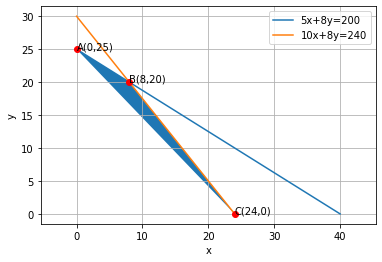
\includegraphics[width=\columnwidth]{Diagram.png}
\caption{Plywood Problem}
\label{fig:Plywood problem}	
\end{figure}
\end{document}
